\documentclass{standalone}
\usepackage{tikz}
\usetikzlibrary{shapes,arrows, positioning,matrix,calc}

\hyphenpenalty=10000
% https://texample.net/tikz/examples/simple-flow-chart/
% Define block styles
\tikzstyle{block} = [rectangle, draw, fill=blue!20, text centered, minimum height=1cm, outer sep=0pt, inner sep=0pt, anchor=north west, text width=3cm]
\tikzstyle{arr} = [-latex', line width=2pt]
% \tikzstyle{arr} = [draw, ->, line width=2pt]

\begin{document}
 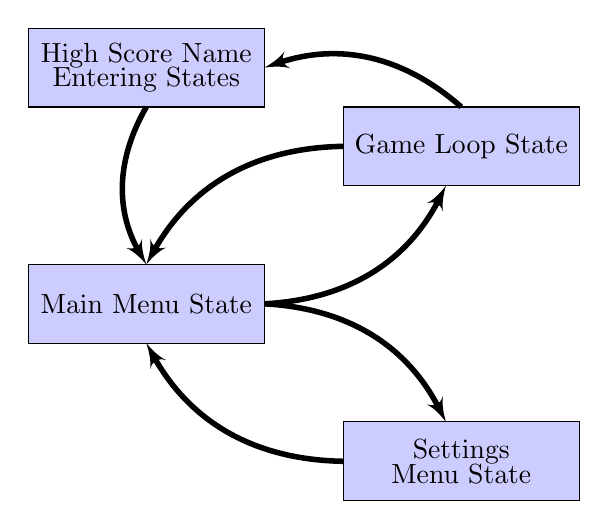
\begin{tikzpicture}[node distance=0cm]
    \renewcommand{\baselinestretch}{0.75}
    \node[block] (main) at (0,0) {Main Menu State};
    \node[block] (sett) at (4,-2)  {Settings Menu State};
    \node[block] (game) at (4,2)  {Game Loop State};
    \node[block] (gamename) at (0,3)  {High Score Name Entering States};

    \path[arr] (main.east) edge[bend left] (sett);
    \path[arr] (main.east) edge[bend right] (game);
    \path[arr] (game.west) edge[bend right] (main.north);
    \path[arr] (sett.west) edge[bend left] (main.south);
    \path[arr] (game.north) edge[bend right] (gamename.east);
    \path[arr] (gamename.south) edge[bend right] (main.north);
    
 \end{tikzpicture}
\end{document}
